\chapter{Core Concepts and State of the Art}

\section{Introduction}

In order to fully understand the inner workings of the eBPF tool and its potential for security and monitoring purposes in data exfiltration scenarios it is important to have a solid understanding of the core concepts of the Linux Kernel and eBPF itself, as well as the current state of the art in security and monitoring tools.
This chapter aims to provide an overview of both of these key topics.



\section{Linux Kernel}
The Linux Kernel is the core component of the Linux operating system \cite{kernel}. It acts as a "bridge" between the hardware and the software layers, it communicates between the two, managing resources as efficiently as possible. 

The jobs of the Linux kernel are:
\begin{enumerate}
    \item \textbf{Process management}
        The kernel determines which processes can use the CPU, and for how long.
    \item \textbf{Memory Management}
        The kernel keeps track of how much memory is used to store what, and where.
    \item \textbf{Device drivers}
        The kernel acts as a mediator between the hardware and the processes.
    \item \textbf{System calls and Security}
        The kernel receives requests for service from processes.
\end{enumerate}


The kernel is quite large, with 30 million lines of code, meaning that performing any change is a challenging task, as making a change to any codebase requires some familiarity with it. Additionally, if the change made locally was to be made part of an official Linux release, it would have to be accepted by the community as a change that would benefit Linux as a whole, taking into account that Linux is a general purpose operating system. Assuming that the change was indeed seen as a net benefit, there would still be a relevant waiting period until it would be accessible to everyone's machine, since most users don't use the Linux kernel directly, but Linux distributions, which use specific versions of the kernel, some of which might be several years old. 


\subsection{System calls}

Applications run in an unprivileged layer called \textit{user space}, which can't access hardware directly. These applications make requests using the system call interface, requesting the kernel to act on its behalf. Since we're more used to the high level abstraction that modern programming languages, we can see an example of just how many system calls are made using the \texttt{strace} utility. For example, using the \texttt{ls} command involves 82 system calls.
%Insert screenshot of strace -c ls
\begin{figure}[h]
    \caption{\texttt{strace} of \texttt{ls} command}
    \centering
    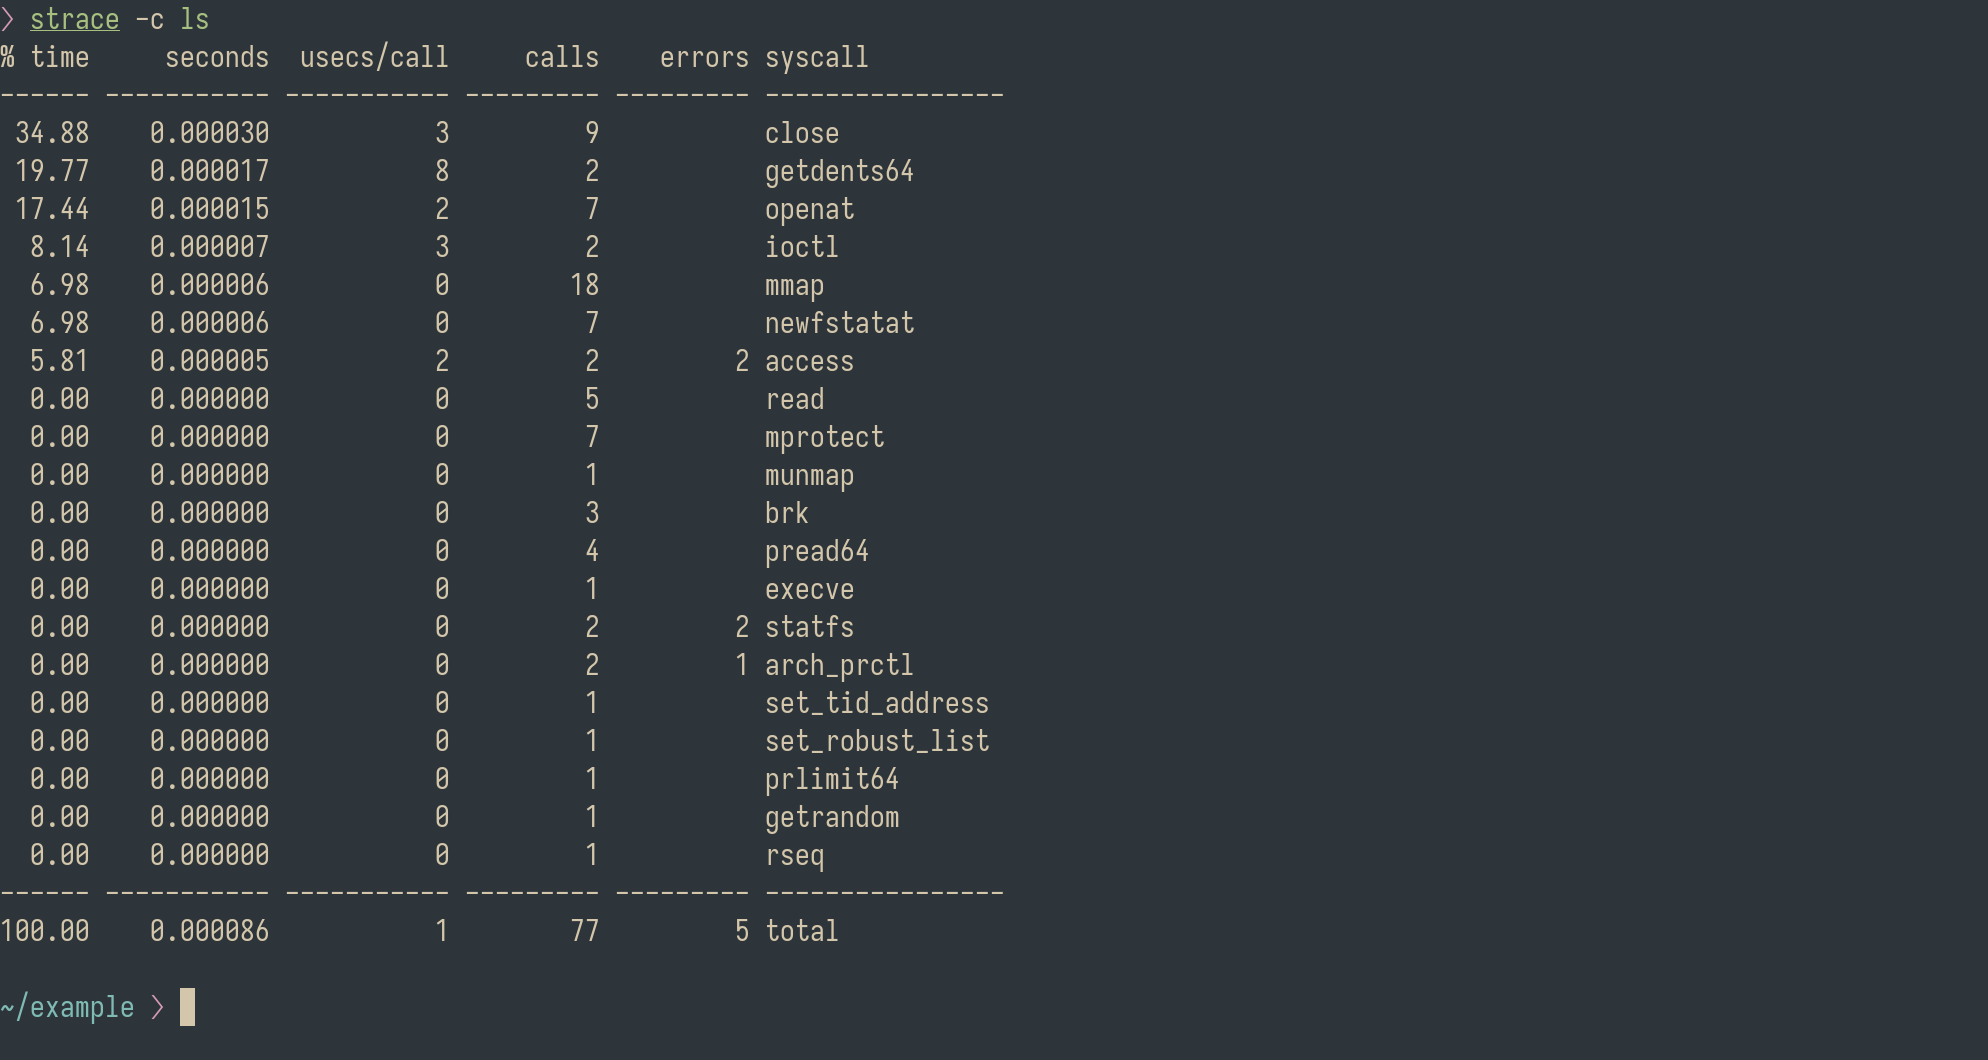
\includegraphics[scale=0.2]{strace}
\end{figure}

Because applications are so heavily reliant on the kernel, it means we can learn a lot by observing its interactions with the kernel. With eBPF we can add instrumentation into the kernel to get these insights, and potentially prevent system calls from being executed.
Assuming we have a user who runs the \texttt{ls} command in a certain directory, eBPF tooling is able to intercept one of the several system calls involved in that command and prevent said command from being run. This makes it quite useful for security purposes, effectively modifying the kernel, running custom code whenever that system call is invoked.

\section{eBPF}

%% Discuss eBPF origins, the changes in recent years in the networking scene, and how LSM BPF makes eBPF a solid and reliable tool for security needs
Extended Berkeley Packet Filter (eBPF) \cite{learningeBPF} originated as an extension of the original Berkeley Packet Filter (BPF), which was designed for packet filtering within the kernel Unix-like operating systems. Although evolving from it, the technology has evolved and is now considered a standalone term. eBPF is a revolutionary technology that allows for developers to write custom code to be loaded into the kernel dynamically, extending the capabilities of the kernel without requiring additional modules or modifications to the kernel source code.

In recent years, eBPF has undergone significant advancements, particularly in the realm of security and monitoring. Its programmability has naturally led to the development of tools and frameworks that leverage its capabilities. eBPF provides deep insights into system activities, allowing for the gain of real-time visibility into the inner workings of the kernel.

From a monitoring perspective, eBPF has revolutionized the way that system monitoring is developed, as it allows for the efficient and secure data collection through the Linux kernel, incurring in less overhead than traditional tools, enabling the monitoring of application processes and system resource usage through system calls, eliminating the need to use monitoring agents in user space. 

Furthermore, in recent years, the eBPF ecosystem has expanded with the development of user-friendly tools and libraries, making it more accessible. As a result, researchers, developers and companies alike can harness the power of eBPF to address specific security concerns. This continuous evolution of eBPF marks it as one of the most exciting recent technologies in the Linux ecosystem.




\textbf{\subsection{eBPF Code}}

Writing eBPF code involves a combination of high level languages and a just-in-time (JIT) compiler, allowing for the creation of efficient and flexible programs that run within the Linux kernel. 

User space programs are used to interact with eBPF from user space, usually written in  high level languages and are responsible for loading eBPF programs into the kernel. This involves compiling the user-written code into eBPF bytecode, verifying its safety and then loading into the kernel using the \texttt{bpf()} system call or any abstraction provided by the language used. User space programs manage the entirety of eBPF programs, attaching or detaching them from hooks dynamically. User space programs can also respond to events triggered by eBPF kernel programs, such as the analysis of network packets, allowing syscalls to be executed, etc. This allows for the development of reactive applications that respond to real-time events in the kernel, making it useful for the detection of data exfiltration as is our objective. 

Kernel space programs are attached to hooks, which are predefined locations in the kernel where eBPF programs can be run, allowing them to intercept and manipulate data at various points in the kernel's execution, as these hooks can be associated with various events, such as system calls, function calls, etc. Kernel side programs are subject to a verification process before being loaded, ensuring the safety of the code, and are then ran inside the eBPF virtual machine within the kernel. 

The communication between user space and kernel space is achieved through the use of pre-defined data structures, known as eBPF maps. These maps are used to pass general information between the user and kernel. Several types of maps are supported, such as array maps, per-CPU maps, hash maps and ring buffers, each being ideal for different use cases. The access of the information held in an eBPF map, from user space, is made through two system calls \texttt{bpf\_map\_lookup\_elem()} and \texttt{bpf\_map\_update\_elem()}, which provide read and write operations on eBPF maps, respectively.

Since eBPF code is kernel specific, a potential limitation is the portability and compatibility across different kernel versions. This limitation is tackled by the CO-RE, (Compile Once - Run Everywhere), approach, aiming to enhance the deployment and maintainability of eBPF programs across different versions. This approach consist of a few key elements:
\begin{enumerate}
    \item \textit{BTF} BPF Type Format serves the purpose of expressing the layout of data structures and function signatures, detecting any differences at compilation time and runtime. 
    \item \textit{Kernel headers} The Linux kernel makes use of header files, which describe the data structures it uses, which can change between versions of the kernel. \texttt{bpftool} allows for the generating of a header file containing all the data structure information that might be needed. 
    \item \textit{Compiler support} The Clang compiler is used to compile eBPF programs with the \texttt{-g} flag. 
    \item \textit{Library support for data structure relocations} \texttt{libbpf} allows for the compensation of any differences between the data structures present at compile time and the ones present at runtime.
    \item \textit{BPF skeleton} A skeleton file, containing helper functions to manage the lifecycle of an eBPF program can be generated using \texttt{bpftool}. This is an optional element in this approach. 
\end{enumerate}
Through this approach an eBPF program can run on different kernel versions, massively improving the portability of eBPF. 

The verification process of an eBPF program consists in the static analysis of it.
It operates in two steps: first, it performs a directed acyclic graph (DAG) check to disallow loops and validate the control flow graph. Then, it simulates the execution of every instruction and observes the state change of registers and the stack to track the range of possible values in each register and stack slot. This is done to ensure that the program is safe to run and does not violate certain safety rules, such as writing outside designated memory regions or performing restricted arithmetic operations on pointers. The eBPF verifier is not a security tool inspecting what the programs are doing, but rather a safety tool checking that programs are safe to run. \cite{verifier}.


\textbf{\subsection{eBPF Programs and Attachment Types}}

eBPF supports several program types and types. Only some are presented, since they total around 30 program types, and more than 40 attachment types. 


\subsubsection{Kfuncs}

\textit{Kfuncs} are functions in the Linux kernel that are exposed for use by eBPF programs. Unlike normal eBPF helpers, \textit{kfuncs} do not have a stable interface and can change from one kernel release to another. They provide an API that eBPF applications can call, but it is less stable than the set of BPF helpers.\cite{kfunc}

\subsubsection{Kprobes and Kretprobes}

\textit{Kprobes} enable you to dynamically break into any kernel routine and collect debugging and performance information non-disruptively. You can trap at almost any kernel code address specifying a handler routine to be invoked when the breakpoint is hit. \cite{kprobe} The main difference between \textit{kprobes} and \textit{kretprobes} is that the latter provides the ability to execute a handler after a specific instruction, which can prove useful to capture the return value of a function.

\subsubsection{Fentry/Fexit}

\textit{Fentry/fexit} are two types of probes that allow for the collection of information, modification of parameters or simply the observation of return values at specific stages of kernel functions execution. \textit{Fentry} is triggered at the entry point of said functions, and \textit{fexit} is triggered at the exit point.

\subsubsection{Tracepoints}

Tracepoints are static markers in the kernel's code that allow developers to attach code in a running kernel. These tracepoints are not exclusive to eBPF and, unlike \textit{kprobes}, are stable between kernel releases.


\subsubsection{User Space Attachments}


User space attachments in eBPF refer to the capability of attaching eBPF programs to user space events, such as user space functions or system calls, for monitoring and tracing purposes. This functionality allows for the dynamic instrumentation of user space applications without requiring modifications to the application's source code or the need for recompilation.

There are considerations and challenges when instrumenting user space code, but despite these challenges, several useful tools leverage eBPF to instrument user space applications. Examples include tracing decrypted versions of encrypted information in the SSL library and continuous profiling of applications.


\subsubsection{LSM}

BPF LSM (Linux Security Module) is a framework in the Linux kernel that allows the dynamic loading of custom eBPF programs to implement security inspection features. It leverages the LSM framework, enabling the attachment of eBPF programs to predefined hook points, allowing for the writing of granular security policies. BPF LSM programs can be attached to LSM hooks using the \texttt{bpf} system call \texttt{BPF\_RAW\_TRACEPOINT\_OPEN} operation. The return value of these programs influences the kernel's behaviour, allowing for the prevention of an operation to be completed. \cite{lsm1} \cite{lsm2}


\begin{comment}
\subsubsection{Networking}

Notably, these program types necessitate specific capabilities, requiring either \texttt{CAP\_NET\_ADMIN} and \texttt{CAP\_BPF} or \texttt{CAP\_SYS\_ADMIN} capabilities to be granted.

The context provided to these programs is the network message under consideration, although the structure of this context depends on the data available at the relevant point in the network stack. At the bottom of the stack, data is represented as Layer 2 network packets—a sequence of bytes prepared or in the process of being transmitted over the network. On the other hand, at the top of the stack where applications interact, sockets are employed, and the kernel generates socket buffers to manage data transmission to and from these sockets.

One big difference between the networking program types and the tracing-related types is that they are generally intended to allow for the customization of networking behaviors. That involves two main characteristics:

\begin{enumerate}
    \item Using a return code from the eBPF program to tell the kernel what to do with a network packet-which could involve processing it as usual, dropping it, or redirecting it to a different destination. 
    \item Allowing the eBPF program to modify network packets, socket configuration parameters.
\end{enumerate}


\subsubsection{Sockets}

In the upper layers of the network stack, specific eBPF program types are dedicated to socket and socket-related operations:

\begin{enumerate}
    \item \textbf{BPF\_PROG\_TYPE\_SOCKET\_FILTER} which is primarily used for filtering a copy of socket data, being useful for sending filtered data to observability tools. 
    \item \textbf{BPF\_PROG\_TYPE\_SOCK\_OPS} which is applied to sockets specific to \texttt{TCP} connections, allowing for the interception of various socket operations and actions, providing the ability to set parameters like TCP timeout values for a socket. 
    \item \textbf{BPF\_PROG\_TYPE\_SK\_SKB} which is utilized in conjunction with a specific map type holding socket references, enabling \texttt{sockmap} operations, facilitating traffic redirection to different destinations at the socket layer.
\end{enumerate}

These program types offer capabilities ranging from filtering socket data for observability to controlling parameters and actions on sockets within Layer 4 connections.

\subsubsection{Traffic control}


Further down the network stack is the TC (traffic control) subsystem in the Linux kernel, which is complex and crucial for providing deep flexibility and configuration over network packet handling. eBPF programs can be attached to the TC subsystem, allowing custom filters and classifiers for both ingress and egress traffic. This is a fundamental component of projects like Cilium. The configuration of these eBPF programs can be done programmatically or using the \texttt{tc} command.


\subsubsection{XDP}

These eBPF programs attach to specific network interfaces, enabling the use of distinct programs for different interfaces. Managing XDP (eXpress Data Path) programs is facilitated through the ip command. The effectiveness of the attachment can be verified using the \texttt{ip link show command}, which provides detailed information about the currently attached XDP program.

\end{comment}


\subsubsection{BPF Attachment Types}

The attachment type plays a crucial role in defining the location within the system where a program can be attached. 
While the attachment type can be automatically determined in some programs based on the hook to which they are attached, others can be attached to multiple points in the kernel, hence an attachment type needs to be explicitly specified. This specification influences the ability to access helper functions and restricts interaction with specific context information.

In instances where a particular attachment type is required, the kernel function \texttt{bpf\_prog\_load\_check\_attach} serves the purpose of validating its appropriateness for specific program types.

To ascertain the valid attachment types applicable to different programs, one can refer to the comprehensive documentation provided by \texttt{libbpf}. This documentation not only outlines recognized section names for each program but also elucidates on the permissible attachment types. The correct understanding and specification of attachment types become imperative when working with eBPF programs, as this knowledge forms the foundation for ensuring the proper integration and behavior of the programs within the kernel.


\section{State of the Art}

Gathering all the information presented above, eBPF presents new capabilities in  the security and observability realm. There already several projects leveraging eBPF to develop security tools.
We will talk about some of these tools, as well as some classical approaches to the prevention of data exfiltration. 

\subsection{Tetragon}

Tetragon \cite{tetragon} is a relatively new tool in the industry, leveraging eBPF's capabilities to detect and react to security relevant events, such as system calls, process execution events and I/O activity in general. 

Tetragon itself is a runtime security enforcement and observability tool, applying policy and filtering directly in eBPF in the kernel. From an observability use case, as we've seen with eBPF, applying filters directly in the kernel reduces observation overhead. This tool provides rich filters in eBPF, allowing users to specify important and relevant events in their specific context. 

Tetragon can also hook into any function in the Linux kernel and filter based on the information this provides. Tetragon also allows for hooking to points where data structures cannot be manipulated by user space applications inside the kernel, effectively solving several common observability and security use cases, such as system calls tracing, where data is incorrectly read, altered or missing due to user/kernel boundary errors. 

Due to the topics discussed above we can conclude that Tetragon is a solid tool for the prevention of data exfiltration, allowing for users to set policies and enforcing those same policies inside the kernel space. One concrete example of this is disallowing certain user/processes to access critical files inside the system, which will then be enforced at the kernel level, preventing and presenting a trace of data exfiltration attempts. Tetragon's approach is mainly to be used in a Kubernetes environment, being that this project defines a custom Kubernetes resource typecalled \textit{TracingPolicy}. 

\begin{figure}
    \centering
    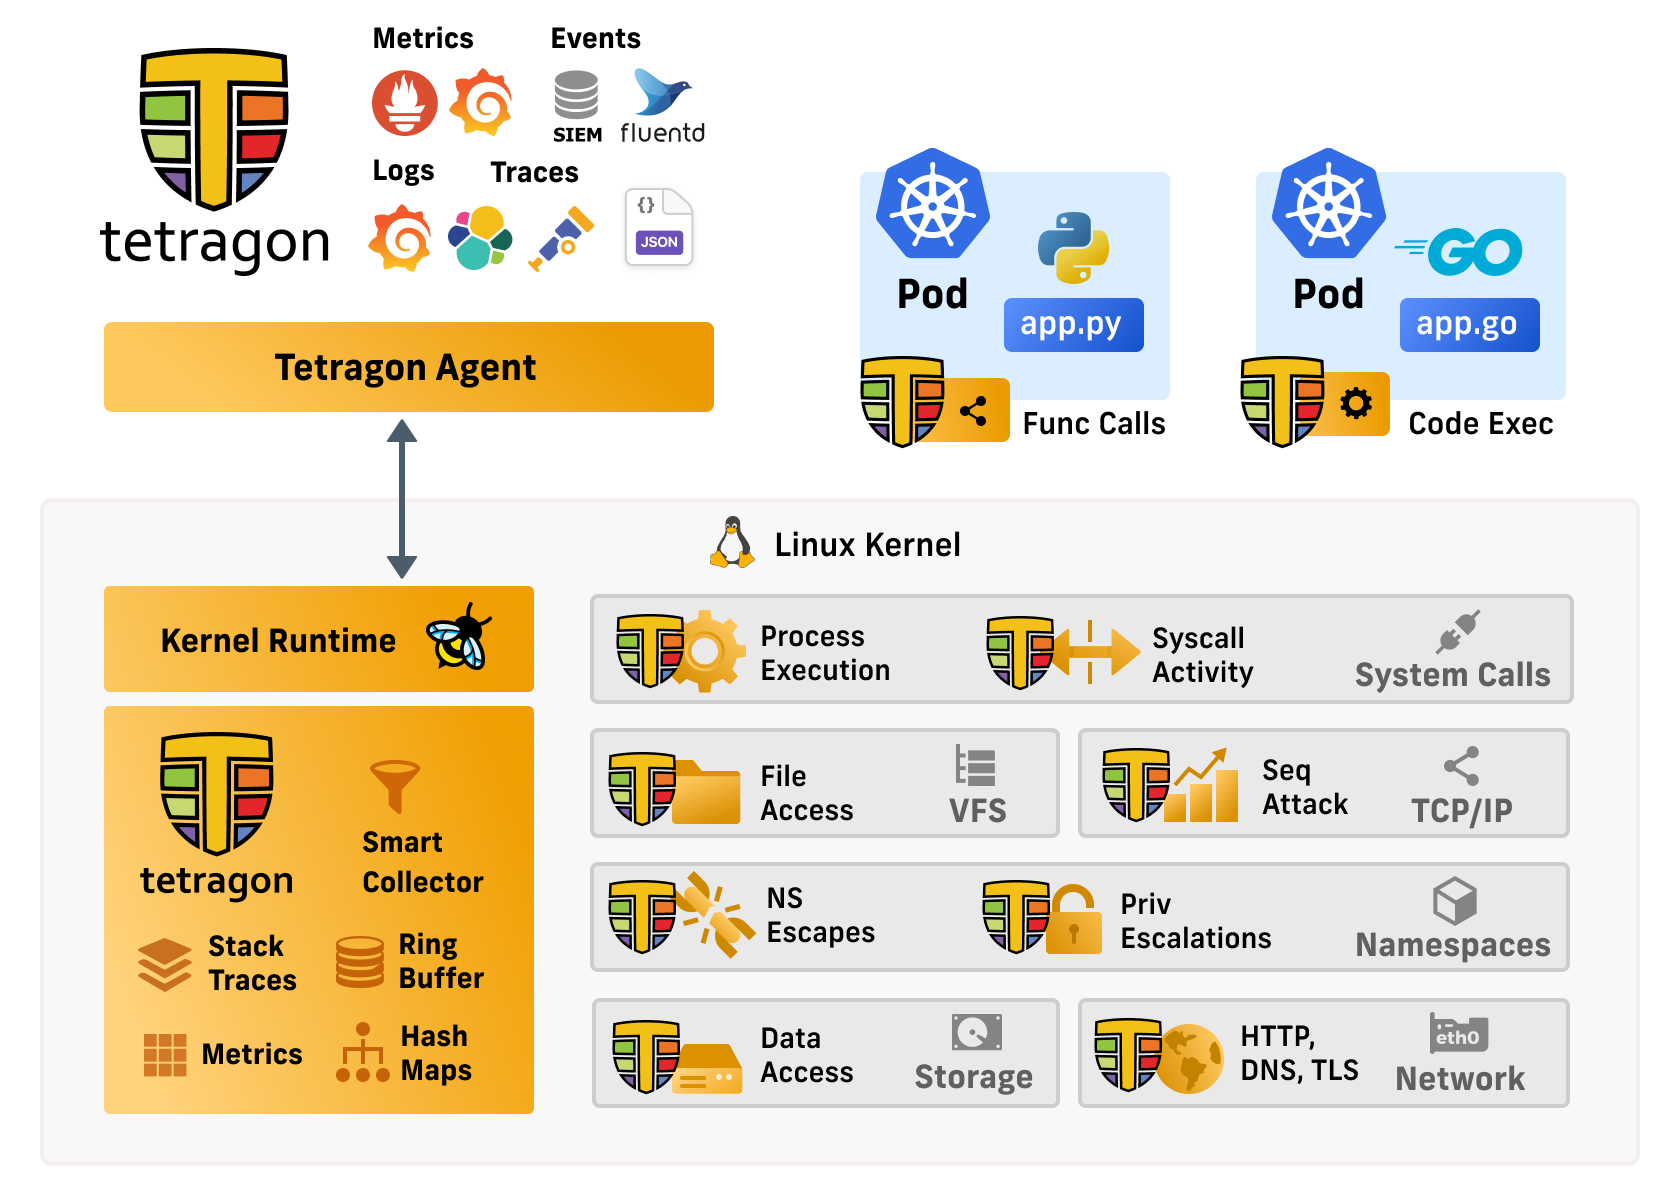
\includegraphics[scale=0.2]{imagens/tetragon.png}
    \caption{Tetragon Overview}
    \label{fig:enter-label}
\end{figure}

\subsection{\textit{Seccomp}}

\textit{Seccomp} \cite{seccomp} \cite{seccomp2}, short for secure computing mode, is a Linux kernel feature that provides a simple and efficiet mechanism for restricting the system calls a process can make. The intention of this tool was to allow users to run untrusted code without any possibility of that code executing malicious tasks. 

One iteration of this tool, known as \texttt{seccomp-bpf}, allows for the filtering of system calls using a configurable BPF program. It provides a means for a process to specify a filter for incoming system calls allowing for expressive filtering of system calls. The filter has access both to the system call and its arguments, taking one of the following actions: 

\begin{enumerate}
    \item Allow the system call. 
    \item Return an error code to the application that made the system call. 
    \item Kill the thread. 
    \item Notify a user space application.
\end{enumerate}

However, since some of the arguments passed to system calls are pointers and the BPF code used in this tool is not able to dereference these pointers, it has limited flexibility, using only value arguments in its decision-making process. It also has to be applied to a process when it starts, making it impossible to modify the profile in real time. 

\subsection{Syscall-Tracking Security Tools}

Numerous tools fall within this category; however, this methodology is susceptible to Time of Check to Time of Use (TOCTOU) issues. When an eBPF program is triggered at the entry point of a system call, it gains access to the arguments passed to that call. Typically, in kernel space, if these arguments are pointers, the kernel copies the data into its own data structures before processing it. During this process, there exists a window of vulnerability wherein an attacker can manipulate the data after inspection but before the kernel completes its copy.

This poses a challenge because the data acted upon may differ from the originally captured data. One potential solution is to attach to both the entry and exit points in system calls. While this approach can provide accurate records of security-relevant events, it cannot prevent an action from occurring, as the system call has already concluded by the time the exit check is conducted.

Therefore, an effective strategy involves attaching the program to an event that occurs after the parameters have been copied into kernel memory, with the understanding that the data is handled differently in system call-specific codes. The prevailing and considered most appropriate approach is leveraging the Linux Security Module.

\subsection{BPF LSM}

The Linux Security Module interface contains certain hookpoints that occur just before the kernel acts on a kernel data structure, triggering a function that can make a decision on whether or not to allow the action to be taken. Originally, this interface allowed for security tools to be implemented as kernel modules, being extended by BPF LSM allowing for the attachment of eBPF programs to the same hook points. 

The fact that the hooks are defined in points where the kernel is about to act on certain arguments, and not the entry point of a specific system call, effectively solves the Time of Check to Time of Use issue, and as such, it is the most correct approach for security tools that aim to provide not only observability but also prevention of security relevant events. 

BPF LSM was added in kernel version 5.7, and as such, it is not yet widely available accross Linux distributions.


\subsection{Formally verified approaches}

As of the writing of this document, no projects or tools leverage formal verification of eBPF code. The closest examples of these were found in a paper where there was the verification of the interpreter of an instruction set closely resembling eBPF. \cite{bpfverif}, and a project where there was an attempt to create a translation validator for BPF programs, written in Coq \cite{bpfproof}. 


\section{Conclusion}
This chapter provides a comprehensive overview of the core concepts of eBPF and the state of the art in eBPF based security tooling. With so many different tools available, it is essential to have a clear and concise way to compare and evaluate them. As the eBPF environment continues to see growth and interest both in the industry and in academia, one can expect for these tools to be continually improving on previous iterations. By gaining a deeper understanding of these tools and the underlying concepts, reasearchers and developers can work towards developing new tools that are more secure, identifying and solving potential problems with the approaches now in use. 
